\chapter{Specifikacija programske potpore}
		
	\section{Funkcionalni zahtjevi}
			
			
			\noindent \textbf{Dionici:}
			
			\begin{packed_enum}
				
				\item Naručitelj (FER)
				\item Razvojni tim
				\item Administrator				
				\item Planinari (korisnici aplikacije)
				\item Zaposlenici planinarskih domova
				
			\end{packed_enum}
			
			\noindent \textbf{Aktori i njihovi funkcionalni zahtjevi:}
			
			
			\begin{packed_enum}
				\item  \underbar{Neregistrirani/neprijavljeni korisnik (inicijator) može:}
				
				\begin{packed_enum}
					
					\item pregledati popis planinarskih staza
					\item pretraživati planinarske staze
					\begin{packed_enum}
						
						\item  prema zemljopisnom položaju 
						\item  prema prosječnom trajanju pješačenja za određenu stazu
						\item  prema zahtjevnosti planinarskog staze
				
					\end{packed_enum}
					\item pregledati popis planinarskih domova
					\item pretraživati planinarske domove
					\begin{packed_enum}
						\item prema dostupnoj infrastrukturi (voda, prenoćište, struja, hrana, internet)
						\item prema zemljopisnom položaju
					\end{packed_enum}
					\item se registrirati u sustav kao planinar tako što popuni formu za registraciju
				\end{packed_enum}
			
				\item  \underbar{Planinar (inicijator) može:}
				
				\begin{packed_enum}
					\item prijaviti se u sustav kao planinar
					\item odjaviti se iz sustava
					\item upravljati vlastitim korisničkim računom
						\begin{packed_enum}
							
							\item  pregledati osobne podatke 
							\item  uređivati osobne podatke
							\item  ukloniti korisnički račun
							
						\end{packed_enum}
					\item pretraživati korisnike prema imenu i prezimenu
					\item upravljati zahtjevima za prijateljstvo
					
						\begin{packed_enum}
							\item poslati zahtjev za prijateljstvom (zahtjev za dodavanjem drugog planinara na popis vlastite planinarske zajednice)
							\item prihvatiti zahtjev za prijateljstvom
							\item pregledati pristigle zahtjeve za prijateljstvom
							\item vidjeti obavijest ako je drugi planinar prihvatio njegov zahtjev
						\end{packed_enum}
					
					\item pregledati popis planinara u vlastitoj planinarskoj zajednici
					\item upravljati vlastitim planinarskim stazama
					\begin{packed_enum}
						\item stvoriti vlastitu planinarsku stazu prema unaprijed određenom predlošku
						\item pregledati staze koje je stvorio
						\item obrisati vlastitu planinarsku stazu ukoliko je ona privatna
					\end{packed_enum}
					\item pregledati popis željenih planinarskih staza (favoriti)
					\item dodati planinarsku stazu na popis željenih
					\item ocjenjivati stvorene planinarske staze drugih planinara
					\item prijaviti netočne i neprecizne informacije vezane uz planinarske staze
					\item stvoriti događaj vidljiv na naslovnici na koji može
						\begin{packed_enum}
							
							\item  pozvati korisnike aplikacije s popisa vlastite planinarske zajednice 
							\item  pregledati popis ljudi koji dolaze na kreirani događaj
							
						\end{packed_enum}
					\item na naslovnici vidjeti nove objave korisnika s popisa vlastite planinarske zajednice
						\begin{packed_enum}
					
							\item  kreirani događaji
							\item  ostvareni bedževi
							
						\end{packed_enum}
					\item dodati ranije odrađene planinarske staze u arhivu
					\item dodati ranije posjećene planinarske domove u arhivu (zatražiti potvrdu od dežurnog planinara da je bio u domu)
					\item obzirom na svoju aktivnost zaraditi određeni bedž koji se prikazuje na njegovom profilu
					\item kontaktirati administratora u slučaju potrebe za stvaranjem novog planinarskog doma ili promjene infrastrukture već postojećeg
				\end{packed_enum}
				
				\item  \underbar{Dežurni planinar (inicijator) može:}
				
				\begin{packed_enum}
					
					\item zatražiti ulogu dežurnog planinara u određenom planinarskom domu  
					\item upravljati zaprimljenim zahtjevima za potvrdom posjeta u planinarskim domovima za koje je odgovoran
					\begin{packed_enum}
						
						\item pregledati zahtjeve
						\item potvrditi ili odbiti zahtjev
						
					\end{packed_enum}
				\end{packed_enum}
			
				\item  \underbar{Administrator (inicijator) može:}
				
				\begin{packed_enum}
					
					\item obrisati korisničke račune
					\item upravljati zaprimljenim zahtjevima za dežurnog planinara
					\begin{packed_enum}
						
						\item pregled zahtjeva
						\item prihvaćanje i odbijanje zahtjeva
					
					\end{packed_enum}
					\item upravljati planinarskim stazama
						\begin{packed_enum}
							\item pregled prijavljenih netočnih i nepreciznih informacija vezanih uz objavljene planinarske staze
							\item uređivanje staza
							\item brisanje staza
						\end{packed_enum}	
					\item upravljati planinarskim domovima
					\begin{packed_enum}
						\item pregled prijavljenih netočnih i nepreciznih informacija vezanih uz objavljene planinarske domove
						\item uređivanje postojećih planinarskih domova
						\item stvaranje novog planinarskog doma
						\item brisanje planinarskih domova
					\end{packed_enum}
					\item pregledati poruke koje su poslali planinari
					
				\end{packed_enum}
	
				\item  \underbar{Baza podataka (sudionik):}
				
					\begin{packed_enum}
						
						\item komunicira s cjelokupnim sustavom
						\item pohranjuje sve podatke nužne za uspješno funkcioniranje sustava
						
					\end{packed_enum}
			\end{packed_enum}
			
			\eject 
			
			
				
			\subsection{Obrasci uporabe}
								
				\subsubsection{Opis obrazaca uporabe}
				
					

				
				\noindent \underbar{\textbf{UC$ $1$ $ -$ $Registracija$ $}}
			\begin{packed_item}
				
				\item \textbf{Glavni sudionik: }$ $Neregistriani korisnik aplikacije (posjetitelj)$ $
				\item  \textbf{Cilj:} $ $Stvaranje novog korisničkog računa s ulogom "planinar"$ $
				\item  \textbf{Sudionici:} $ $Baza podataka$ $
				\item  \textbf{Preduvjet:} $ $/$ $
				\item  \textbf{Opis osnovnog tijeka:}
				
				\item[] \begin{packed_enum}
					
					\item $ $Neregistrirani korisnik pokrene aplikaciju$ $
					\item $ $Neregistrirani korisnik odabere opciju za registraciju te unosi osobne podatke$ $
					\item $ $Sustav validira podatke te ih sprema u bazu podataka u slučaju ispravnosti$ $
					\item $ $Korisnik prima obavijest o uspješnoj registraciji$ $
				\end{packed_enum}
				
				\item  \textbf{Opis mogućih odstupanja:}
				
				\item[] \begin{packed_item}
					
					\item[3.a] $ $Unos e-maila koji se već koristi, unos e-maila koji ne zadovoljava propisani format e-maila, neispunjavanje svih potrebnih polja forme za registraciju, lozinka i ponovljena lozinka se ne podudaraju ili lozinka ne zadovoljava minimalne zahtjeve prihvatljivosti$ $
					
					\item[] \begin{packed_enum}
						
						\item $ $Sustav obavještava korisnika o neispravnim poljima te ostaje na istoj stranici registracije, sva polja forme za registraciju ostaju popunjena unešenim podacima, osim lozinke koju je nužno ponovno unijeti$ $
						\item $ $Korisnik ispravi neispravne podatke te završava unos ili odustaje od registracije$ $
						
					\end{packed_enum}
				\end{packed_item}
			\end{packed_item}
		
			\noindent \underbar{\textbf{UC$ $2$ $ -$ $Prijava$ $}}
		\begin{packed_item}
			
			\item \textbf{Glavni sudionik: }$ $Registrirani korisnik $ $
			\item  \textbf{Cilj:} $ $Pristup korisničkom računu i svim funkcionalnostima aplikacije namijenjenih ulozi koju posjeduju$ $
			\item  \textbf{Sudionici:} $ $Baza podataka$ $
			\item  \textbf{Preduvjet:} $ $Korisik je registriran u sustav kao planinar$ $
			\item  \textbf{Opis osnovnog tijeka:}
			
			\item[] \begin{packed_enum}
				
				\item $ $Korisnik odabere opciju za prijavu$ $
				\item $ $Korisnik unosi ispravan e-mail i lozinku$ $
				\item $ $Prijava je uspješno obavljena i otvara se naslovna stranica$ $
				
			\end{packed_enum}
			
			\item  \textbf{Opis mogućih odstupanja:}
			
			\item[] \begin{packed_item}
				
				\item[3.a] $ $Neispravno korisničko ime i/ili lozinka $ $
				\item[] \begin{packed_enum}
					
					\item $ $Sustav javlja pogrešku, ostaje na istoj stranici za prijavu te očisti sva polja forme za prijavu$ $
				\end{packed_enum}
			\end{packed_item}
		\end{packed_item}
	
			\noindent \underbar{\textbf{UC$ $3$ $ -$ $Odjava$ $}}
		\begin{packed_item}
			
			\item \textbf{Glavni sudionik: }$ $Registrirani korisnik $ $
			\item  \textbf{Cilj:} $ $Odjaviti se sa svog korisničkog profila$ $
			\item  \textbf{Sudionici:} $ $Baza podataka$ $
			\item  \textbf{Preduvjet:} $ $Korisik je prijavljen u sustav$ $
			\item  \textbf{Opis osnovnog tijeka:}
			
			\item[] \begin{packed_enum}
				
				\item $ $Korisnik odabere opciju za odjavu iz sustava$ $
				\item $ $Sustav odjavljuje korisnika, preusmjerava ga na nasolvnu stranicu i dodijeli mu ulogu \underbar{gost}$ $
				
			\end{packed_enum}
		\end{packed_item}
		
			\noindent \underbar{\textbf{UC$ $4$ $ -$ $Pretraživanje planinarskih staza$ $}}
		\begin{packed_item}
			
			\item \textbf{Glavni sudionik: }$ $Korisnik$ $
			\item  \textbf{Cilj:} $ $Pretražiti postojeće planinarske staze prema unaprijed određenim kriterijima $ $
			\item  \textbf{Sudionici:} $ $Baza podataka$ $
			\item  \textbf{Preduvjet:} $ $/$ $
			\item  \textbf{Opis osnovnog tijeka:}
			
			\item[] \begin{packed_enum}
				
				\item $ $Korisnik odabire opciju pretraživanja planinarskih staza$ $
				\item $ $Otvara se stranica za pretragu planinarskih staza s više načina pretraživanja$ $
					\begin{packed_enum}
						\item Prema nazivu staze
						\item Prema zemljopisnom položaju
						\item Prema prosječnom trajanju i/ili zahtjevnosti
					\end{packed_enum}
				\item $ $Korisnik odabire način pretraživanja te odabire gumb za pretragu$ $
				\item $ $Sustav dohvaća sve podatke iz baze podataka koji zadovoljavaju upit pretrage $ $
				\item $ $Prikazuju se postojeće staze koje ispunjavaju zahtjeve pretrage$ $
				
			\end{packed_enum}
		\end{packed_item}
		
		
			\noindent \underbar{\textbf{UC$ $5$ $ -$ $Pretraživanje planinarskih domova$ $}}
		\begin{packed_item}
			
			\item \textbf{Glavni sudionik: }$ $Korisnik$ $
			\item  \textbf{Cilj:} $ $Pretražiti postojeće planinarske domove prema unaprijed određenim kriterijima$ $
			\item  \textbf{Sudionici:} $ $Baza podataka$ $
			\item  \textbf{Preduvjet:} $ $/$ $
			\item  \textbf{Opis osnovnog tijeka:}
			
			\item[] \begin{packed_enum}
				
				\item $ $Korisnik odabire opciju za pregled i pretraživanje planinarskih domova$  $
				\item $ $Otvara se stranica za pretragu planinarskih domova s više načina pretraživanja$ $
				\begin{packed_enum}
					\item Prema zemljopisnom položaju
					\item Prema dostupnoj infrastrukturi (hrana, pitka voda, prenoćište, internet)
				\end{packed_enum}$ $
				\item $ $Korisnik odabire kategoriju pretrage i/ili unosi naziv doma $ $
				\item $ $Sustav dohvaća sve podatke iz baze podataka koji zadovoljavaju upit pretrage $ $
				\item $ $Prikazuju se postojeći planinarski domovi koji ispunjavaju zahtjeve pretrage$ $
				
			\end{packed_enum}
		\end{packed_item}
	
			\noindent \underbar{\textbf{UC$ $6$ $ -$ $Pregled korisničkog računa$ $}}
		\begin{packed_item}
			
			\item \textbf{Glavni sudionik: }$ $Korisnik$ $
			\item  \textbf{Cilj:} $ $Omogućiti korisniku pregled svojih osobnih podataka$ $
			\item  \textbf{Sudionici:} $ $Baza podataka$ $
			\item  \textbf{Preduvjet:} $ $Korisnik prijavljen u sustav$ $
			\item  \textbf{Opis osnovnog tijeka:}
			
			\item[] \begin{packed_enum}
				
				\item $ $Korisnik odabire opciju "Moj profil"$ $
				\item $ $Prikazuje se profil korisnika s njegovim osobnim podacima$ $
				
			\end{packed_enum}
		\end{packed_item}
		
		
		\noindent \underbar{\textbf{UC$ $6.1$ $ -$ $Izmjena korisničkog računa$ $}}
		\begin{packed_item}
			
			\item \textbf{Glavni sudionik: }$ $Registrirani korisnik$ $
			\item  \textbf{Cilj:} $ $Izmjena osobnih podataka$ $
			\item  \textbf{Sudionici:} $ $Baza podataka$ $
			\item  \textbf{Preduvjet:} $ $Korisnik prijavljen u sustav$ $
			\item  \textbf{Opis osnovnog tijeka:}
			
			\item[] \begin{packed_enum}
				
				\item $ $Korisnik odabire opciju "Moj profil" $ $
				\item $ $Prikazuju se korisnički podaci planinara$ $
				\item $ $Korisnik odabire opciju "Uredi osobne podatke"$ $
				\item $ $Sustav prikazuje podatke korisnika u sučelju prigodnom za promjenu$ $
				\item $ $Korisnik promijeni podatke i potvrđuje promjene odabirom opcije "Spremi"$ $
				\item $ $Sustav sprema promijenjene podatke u bazu podataka te prikazuje obavijest korisniku o uspješnoj promjeni podataka $ $
				
			\end{packed_enum}
		\end{packed_item}
		
		
			\noindent \underbar{\textbf{UC$ $6.2$ $ -$ $Uklanjanje korisničkog računa$ $}}
		\begin{packed_item}
			
			\item \textbf{Glavni sudionik: }$ $Planinar$ $
			\item  \textbf{Cilj:} $ $Izbrisati vlastiti korisnički račun $ $
			\item  \textbf{Sudionici:} $ $Baza podataka$ $
			\item  \textbf{Preduvjet:} $ $Korisnik prijavljen u sustav$ $
			\item  \textbf{Opis osnovnog tijeka:}
			
			\item[] \begin{packed_enum}
				
				\item $ $Korisnik odabire opciju "Moj profil"$ $
				\item $ $Prikazuju se korisnički podaci planinara$ $
				\item $ $Korisnik odabire opciju "Ukloni račun" $ $
				\item $ $Sustav uklanja korisnički račun iz baze podataka$ $
				\item $ $Sustav preusmjerava korisnika na naslovnu stranicu$ $
				
			\end{packed_enum}
		\end{packed_item}
	
		\noindent \underbar{\textbf{UC$ $7$ $ -$ $Pretraživanje korisnika po imenu i prezimenu $ $}}
		\begin{packed_item}
			
			\item \textbf{Glavni sudionik: }$ $Planinar$ $
			\item  \textbf{Cilj:} $ $Provjeriti posjeduje li određeni planinar korisnički račun, pronaći poznanike planinare$ $
			\item  \textbf{Sudionici:} $ $Baza podataka$ $
			\item  \textbf{Preduvjet:} $ $Korisnik prijavljen u sustav$ $
			\item  \textbf{Opis osnovnog tijeka:}
			
			\item[] \begin{packed_enum}
				
				\item $ $Korisnik se nalazi na zidu vlastite planinarske zajednice i odabire polje za pretragu drugih korisnika$ $
				\item $ $Sustav omogućava unos podataka za pretragu$ $
				\item $ $Korisnik upisuje ime i/ili prezime željenog planinara$ $	
				\item $ $Sustav dohvaća podatke iz baze podataka koji odgovaraju postavljenom upitu$ $
				\item $ $Sustav prikazuje dohvaćene podatke korisniku $ $
			\end{packed_enum}
		\end{packed_item}
	
		%		\noindent \underbar{\textbf{UC$ $8$ $ -$ $Pregledavanje profila drugog planinara$ $}}
	%		\begin{packed_item}
	%			
	%			\item \textbf{Glavni sudionik: }$ $Planinar$ $
	%			\item \textbf{Cilj:} $ $Pregledati profil drugog planinara (njegove podatke dostupne svim prijavljenim korisnicima)$ $
	%			\item  \textbf{Sudionici:} $ $Baza podataka$ $
	%			\item  \textbf{Preduvjet:} $ $Korisnik prijavljen u sustav$ $
	%			\item  \textbf{Opis osnovnog tijeka:}
	%			
	%			\item[] \begin{packed_enum}
	%				
	%				\item $ $Korisnik pretražuje planinare unoseći njihovo ime i prezime (\textbf{UC6})$ $
	%				\item $ $Korisnik odabire jedan od više mogućih rezultata pretraživanja$ $
	%				\item $ $Sustav dohvaća podatke iz baze podataka za odabranog planinara $ $
	%				\item $ $Sustav preusmjerava korisnika na profil odabranog planinara i prikazuje mu dohvaćene podatke u odgovarajućem obliku$ $	
	%			\end{packed_enum}
	%		\end{packed_item}
	
			\noindent \underbar{\textbf{UC$ $8$ $ -$ $Stvoriti planinarsku stazu$ $}}
			\begin{packed_item}
				
				\item \textbf{Glavni sudionik: }$ $Planinar$ $
				\item  \textbf{Cilj:} $ $Stvoriti novu stazu prema unaprijed određenom predlošku i dodati je na popis postojećih planinarskih staza$ $
				\item  \textbf{Sudionici:} $ $Baza podataka$ $
				\item  \textbf{Preduvjet:} $ $Korisnik prijavljen u sustav$ $
				\item  \textbf{Opis osnovnog tijeka:}
				
				\item[] \begin{packed_enum}
					
					\item $ $Planinar odabire opciju "Stvori novu stazu"$ $
					\item $ $Sustav prikazuje stranicu s odgovarajućom predloškom za unos staze$ $
					\item $ $Planinar ispunjava formu za dodavanje planinarske staze$ $
					\begin{packed_enum}
						\item Unosi naziv staze
						\item Unosi početnu i završnu točku te duljinu staze
						\item Unosi razliku nadmorskih visina početne i završne točke
						\item Unosi zemljopisno područje staze (npr. planina na kojoj se staza nalazi)
						\item Podrazumijevani scenarij je da planinar stazu želi objaviti kao javnu
					\end{packed_enum}	
					\item $ $Sustav dodaje stazu na popis postojećih planinarskih staza$ $
				\end{packed_enum}
				\item  \textbf{Opis mogućih odstupanja:}
				
				\item[] \begin{packed_item}
					
					\item[3.a] $ $Planinar unese neispravne/nepotpune podatke$ $
					\item[] \begin{packed_enum}
						
						\item $ $Dobiva obavijest o neispravnim poljima$ $
						\item $ $Planinar ispravi neispravna polja i završi unos ili odustane od dodavanja nove planinarske staze$ $
					\end{packed_enum}
					\item[4.a] $ $Postoji staza s istim imenom$ $
					\item[] \begin{packed_enum}
						\item $ $Planinar dobiva obavijest da je staza već postojeća te ostaje na istoj formi za unos staze s mogućnošću izmjene unešenih podataka$ $
					\end{packed_enum}
					\item[5.a] $ $Planinar označava stazu kao privatnu$ $
					\item[] \begin{packed_enum}
						\item $ $ Staza ostaje vidljiva samo planinaru koji ju je stvorio $ $
					\end{packed_enum}
				\end{packed_item}
			\end{packed_item}
			
			\noindent \underbar{\textbf{UC$ $9$ $ -$ $Obrisati vlastitu planinarsku stazu$ $}}
			\begin{packed_item}
				
				\item \textbf{Glavni sudionik: }$ $Planinar$ $
				\item  \textbf{Cilj:} $ $Obrisati vlastite staze$ $
				\item  \textbf{Sudionici:} $ $Baza podataka$ $
				\item  \textbf{Preduvjet:} $ $Korisnik prijavljen u sustav$ $
				\item  \textbf{Opis osnovnog tijeka:}
				
				\item[] \begin{packed_enum}
					
					\item $ $Planinar odabire na profilu odabire opcije "Moje staze"$ $
					\item $ $Sustav prikazuje popis staza koje je stvorio trenutni korisnik$ $
					\item $ $Korisnik pronalazi stazu koju želi ukloniti te odabire opciju "Ukloni stazu"$ $	
					\item $ $Sustav postavlja poruku "Jeste li sigurni da želite obrisati stazu?"$ $
					\item $ $Korisnik potvrđuje te sustav obavještava korisnika da je staza uspješno obrisana $ $
				\end{packed_enum}
				\item  \textbf{Opis mogućih odstupanja:}
				
				\item[] \begin{packed_item}
					
					\item[3.a] $ $Korisnik se predomišlja i ne želi obrisati stazu$ $
					\item[] \begin{packed_enum}
						
						\item $ $Sustav vraća korisnika na popis vlastitih staza$ $
						\end{packed_enum}
					\item[4.a] $ $Staza koju korisnik pokušava obrisati je javna$ $
					\item[] \begin{packed_enum}
						\item $ $Sustav obavještava korisnika da se javne staze ne mogu obrisati$ $
					\end{packed_enum}
				\end{packed_item}
			\end{packed_item}
			
	
	
			\noindent \underbar{\textbf{UC$ $10$ $ -$ $Slanje zahtjeva za prijateljstvom$ $}}
		\begin{packed_item}
			
			\item \textbf{Glavni sudionik: }$ $Planinar$ $
			\item  \textbf{Cilj:} $ $Poslati zahtjev za pridruživanjem vlastitoj planinarskoj zajednici drugom planinaru (zahtjev za prijateljstvom) $ $
			\item  \textbf{Sudionici:} $ $Baza podataka, Planinar$ $
			\item  \textbf{Preduvjet:} $ $Pošiljatelj i primatelj zahtjeva (planinari) posjeduju korisnički račun$ $
			\item  \textbf{Opis osnovnog tijeka:}
			
			\item[] \begin{packed_enum}
				
				\item $ $Korisnik pronađe željenog planinara prema obrascu \textbf{UC7}$ $
				%\item $ $Korisnik odlazi na profil odabranog planinara prema obrascu \textbf{UC8}$ $
				\item $ $Nakon prikaza korisnika koji zadovoljavaju pretragu planinar odabire opciju "Zahtjev za prijateljstvom"$ $
				\item $ $Sustav prikazuje poruku pošiljatelju da je zahtjev uspješno poslan te obavještava primatelja da ima novi zahtjev $ $	
			\end{packed_enum}
		\end{packed_item}
	
		\noindent \underbar{\textbf{UC$ $11$ $ -$ $Pregledavanje pristiglih zahtjeva za prijateljstvo$ $}}
		\begin{packed_item}
			
			\item \textbf{Glavni sudionik: }$ $Planinar$ $
			\item  \textbf{Cilj:} $ $Planinar može vidjeti sve trenutno aktivne zahtjeve za prijateljstvo $ $
			\item  \textbf{Sudionici:} $ $Baza podataka $ $
			\item  \textbf{Preduvjet:} $ $Korisnik je prijavljen u sustav$ $
			\item  \textbf{Opis osnovnog tijeka:}
			
			\item[] \begin{packed_enum}
				
				\item $ $Planinaru stiže obavijest da je primio novi zahtjev za prijateljstvom ili želi pregledati pristigle zahtjeve za prijateljstvom $ $
				\item $ $Planinar odabire opciju pregleda pristiglih zahtjeva za prijateljstvom koja se nalazi na zaglavlju stranice$ $
				\item $ $Otvara se popis pristiglih zahtjeva za prijateljstvom čiji je status još uvijek aktivan$ $
				
			\end{packed_enum}
		\end{packed_item}
	
		\noindent \underbar{\textbf{UC$ $11.1$ $ -$ $Prihvatiti zahtjev za prijateljstvom$ $}}
		\begin{packed_item}
			
			\item \textbf{Glavni sudionik: }$ $Planinar$ $
			\item  \textbf{Cilj:} $ $Prihvatiti zahtjev za pridruživanjem planinarskoj zajednici drugog planinara$ $
			\item  \textbf{Sudionici:} $ $Baza podataka, planinar$ $
			\item  \textbf{Preduvjet:} $ $Oba korisnika imaju korisnički račun, jedan korisnik je drugom poslao zahtjev za pridruživanjem vlastitoj planinarskoj zajednici$ $
			\item  \textbf{Opis osnovnog tijeka:}
			
			\item[] \begin{packed_enum}
				
				\item $ $Planinaru stiže obavijest da je primio novi zahtjev za prijateljstvom koja se pokazuje na zaglavlju stranice pod opcijom "Pristgli zahtjevi"$ $
				\item $ $Planinar potvrđuje zahtjev za prijateljstvo te se on uklanja s popisa$ $
				\item $ $Na popis planinarske zajednice obojice planinara dodan je novi član ("prijatelj")$ $
				
			\end{packed_enum}
			
			\item  \textbf{Opis mogućih odstupanja:}
			
			\item[] \begin{packed_item}
				
				\item[2.a] $ $Planinar može odbiti zahtjev za prijateljstvom $ $
				\item[] \begin{packed_enum}
					
					\item $ $Zahtjev za prijateljstvom se uklanja s popisa pristiglih zahtjeva $ $
					\item $ $Odbijeni planinar ima mogućnost ponovnog slanja zahtjeva za prijateljstvo planinaru koji ga je odbio $ $
					
				\end{packed_enum}
			\end{packed_item}
		\end{packed_item}
	
		\noindent \underbar{\textbf{UC$ $12$ $ -$ $Pregled prihvaćenih zahtjeva$ $}}
		\begin{packed_item}
			
			\item \textbf{Glavni sudionik: }$ $Planinar$ $
			\item  \textbf{Cilj:} $ $Planinar može vidjeti sve zahtjeve za prijateljstvom koje su mu prihvatili drugi planinari $ $
			\item  \textbf{Sudionici:} $ $Baza podataka $ $
			\item  \textbf{Preduvjet:} $ $Korisnik je prijavljen u sustav$ $
			\item  \textbf{Opis osnovnog tijeka:}
			
			\item[] \begin{packed_enum}
				
				\item $ $Planinaru stiže obavijest da je netko prihvatio njegov zahtjev za prijateljstvom ili planinar želi vidjeti sve prihvaćene zahtjeve za prijateljstvom$ $
				\item $ $Planinar odabire opciju pregleda pristiglih zahtjeva za prijateljstvom koja se nalazi na zaglavlju stranice$ $
				\item $ $Otvara se popis zahtjeva koje su trenutnom planinaru prihvatili ostali planinari$ $
				
			\end{packed_enum}
		\end{packed_item}

			\noindent \underbar{\textbf{UC$ $13$ $ -$ $Pregled vlastitih planinarskih staza$ $}}
		\begin{packed_item}
			
			\item \textbf{Glavni sudionik: }$ $Planinar$ $
			\item  \textbf{Cilj:} $ $Omogućiti pregled svih staza koje je planinar stvorio$ $
			\item  \textbf{Sudionici:} $ $Baza podataka$ $
			\item  \textbf{Preduvjet:} $ $Korisnik prijavljen u sustav$ $
			\item  \textbf{Opis osnovnog tijeka:}
			
			\item[] \begin{packed_enum}
				\item $ $Planinar odlazi na svoj profil odabirom opcije "Moj profil"$ $
				\item $ $Planinar na svom profilu odabire opciju "Moje staze"$ $
				\item $ $Sustav dohvaća sve staze iz baze podataka koje je stvorio planinar te ih prikazuje u odgovarajućem obliku$ $
			\end{packed_enum}
		\item  \textbf{Opis mogućih odstupanja:}
			\item[] \begin{packed_item}
				
				\item[3.a] $ $Planinar nema nijednu stvorenu stazu$ $
				\item[] \begin{packed_enum}
					\item $ $Prikazuje se odgovarajuća poruka te se nudi opcija za stvaranje vlastite staze$ $
				\end{packed_enum}
			\end{packed_item}
		\end{packed_item}
	
			\noindent \underbar{\textbf{UC$ $14$ $ -$ $Stvoriti događaj$ $}}
		\begin{packed_item}
			
			\item \textbf{Glavni sudionik: }$ $Planinar$ $
			\item  \textbf{Cilj:} $ $Stvoriti novi događaj koji će biti vidljiv svim korisnicima s popisa planinarske zajednice kreatora događaja$ $
			\item  \textbf{Sudionici:} $ $Baza podataka, članovi planinarske zajednice kreatora događaja (pozvani planinari)$ $
			\item  \textbf{Preduvjet:} $ $Korisnik prijavljen u sustav$ $
			\item  \textbf{Opis osnovnog tijeka:}
			
			\item[] \begin{packed_enum}
				
				\item $ $Planinar odabire opciju "Organiziraj događaj" na zidu njegove planinarske zajednice$ $
				\item $ $Sustav preusmjerava korisnika na stranicu s unaprijed pripremljenim predloškom za stvaranje događaja$ $
				\item $ $Planinar ispunjava popunjava predložak za stvaranje događaja$ $	
				\item $ $Sustav stvara novi događaj i sprema ga u bazu podataka$ $
				\item $ $Stvoreni događaj vidljiv je svim članovima planinarske zajednice organizatora$ $ 
			\end{packed_enum}
			\item  \textbf{Opis mogućih odstupanja:}
			
			\item[] \begin{packed_item}
				
				\item[3.a] $ $Planinar unosi nepotpune podatke$ $
				\item[] \begin{packed_enum}
					\item $ $Na predlošku se ispisuju poruke pogreške$ $
					\item $ $Planinar ispravi neispravna polja i završi unos ili odustane od stvaranja novog događaja$ $
				\end{packed_enum}
			\end{packed_item}
		\end{packed_item}
	
		\noindent \underbar{\textbf{UC$ $15$ $ -$ $Sudjelovati u događajima planinarske zajednice$ $}}
		\begin{packed_item}
			
			\item \textbf{Glavni sudionik: }$ $Planinar$ $
			\item  \textbf{Cilj:} $ $Događaje stvorene u vlastitoj planinarskoj zajednici označiti s "Dolazim"$ $
			\item  \textbf{Sudionici:} $ $Baza podataka$ $
			\item  \textbf{Preduvjet:} $ $Korisnik prijavljen u sustav s ulogom \underbar{planinar}$ $
			\item  \textbf{Opis osnovnog tijeka:}
			
			\item[] \begin{packed_enum}
				
				\item $ $Planinar odlazi na zid objava vlastite planinarske zajednice$ $
				\item $ $Planinar pregledava stvorene događaje te određeni događaj označi sa "Dolazim"$ $
				\item $ $Sustav pohranjuje njegovu odluku u bazu podataka$ $	
				\item $ $Planinar je dodan na popis ljudi koji dolaze na odabrani događaj$ $ 
			\end{packed_enum}
			\item  \textbf{Opis mogućih odstupanja:}
				
			\item[] \begin{packed_item}
				
				\item[3.a] $ $Planinar je shvatio da ipak ne može doći na odabrani događaj$ $
				\item[] \begin{packed_enum}
					\item $ $Na konkretnom događaju odabire opciju "Otkaži dolazak"$ $
					\item $ $Sustav uklanja planinara s popisa ljudi koji dolaze na događaj$ $
				\end{packed_enum}
			\end{packed_item}
		\end{packed_item}
	
		\noindent \underbar{\textbf{UC$ $16$ $ -$ $Zahtjev za dodjeljivanje uloge "dežurni planinar"$ $}}
		\begin{packed_item}
			
			\item \textbf{Glavni sudionik: }$ $Planinar$ $
			\item  \textbf{Cilj:} $ $Dodjela uloga "dežurnog planinara" planinaru koji je tu ulogu zatražio$ $
			\item  \textbf{Sudionici:} $ $Baza podataka, Administrator$ $
			\item  \textbf{Preduvjet:} $ $Korisnik prijavljen u sustav s ulogom \underbar{planinar}$ $ 
			\item  \textbf{Opis osnovnog tijeka:}
			
			\item[] \begin{packed_enum}
				
				\item $ $Planinar pretražuje planinarski dom za koji želi biti dežurni te se prijavi za dežurnog planinara odabirom opcije "Dežurni planinar"$ $
				\item $ $Sustav proslijedi zahtjev \underbar{Administratoru}$ $
				\item $ $Administrator dodjeljuje ulogu \underbar{dežurnog planinara} planinaru koji je poslao zahtjev prema obrascu \textbf{UC18}$ $
				\item $ $Nakon prihvaćanja zahtjeva dežurni planinar vidi sve zahtjeve za posjetom za zatraženi dom$ $
			\end{packed_enum}
		\item  \textbf{Opis mogućih odstupanja:}
		
		\item[] \begin{packed_item}
			
			\item[3.a] $ $Administrator odbija dodijeliti ulogu dežurnog planinara$ $
			\item[] \begin{packed_enum}
				\item $ $Sustav uklanja zahtjev s popisa zahtjeva za dežurnog planinara na profilu administratora$ $
				\item $ $Planinaru se omogućuje ponovna prijava za "dežurnog planinara" za konkretni planinarski dom $ $
			\end{packed_enum}
		\end{packed_item}
		\end{packed_item}
	
			\noindent \underbar{\textbf{UC$ $17$ $ -$ $Pregled zahtjeva za dežurnog planinara$ $}}
		\begin{packed_item}
			
			\item \textbf{Glavni sudionik: }$ $Administrator$ $
			\item  \textbf{Cilj:} $ $Pregledati pristigle zahtjeve za dežurnog planinara$ $
			\item  \textbf{Sudionici:} $ $Baza podataka$ $
			\item  \textbf{Preduvjet:} $ $Korisnik prijavljen u sustav s ulogom \underbar{administrator} $ $
			\item  \textbf{Opis osnovnog tijeka:}
			
			\item[] \begin{packed_enum}
				
				\item $ $Administrator na vlastitom profilu odabire opciju "Zahtjevi za dežurnog planinara"$ $
				\item $ $Sustav dohvaća iz baze podataka sve zahtjeve za dežurnog planinara te ih prikazuje u odgovarajućem obliku$ $
			\end{packed_enum}
		\end{packed_item}
		
		\noindent \underbar{\textbf{UC$ $18$ $ -$ $Prihvatiti/odbiti zahtjev za dežurnog planinara$ $}}
		\begin{packed_item}
			
			\item \textbf{Glavni sudionik: }$ $Administrator$ $
			\item  \textbf{Sudionici:} $ $Baza podataka, Planinar (koji je zatražio zahtjev)$ $
			\item  \textbf{Preduvjet:} $ $Korisnik prijavljen u sustav s ulogom \underbar{administrator}$ $
			\item  \textbf{Opis osnovnog tijeka:}
			
			\item[] \begin{packed_enum}
				
				\item $ $Administrator pregledava zahtjeve za dežurnog planinara prema obrascu \textbf{UC17} $ $
				\item $ $Administrator prihvaća zahtjev za dežurnog planinara$ $
				\item $ $Sustav sprema novonastalu vezu između planinara i planinarskog doma u bazu podataka$ $
				\item $ $Planinaru kojem je zahtjev potvrđen se na popis domova dodaje traženi dom$ $
				
				
			\end{packed_enum}
			\item  \textbf{Opis mogućih odstupanja:}
			
			\item[] \begin{packed_item}
				
				\item[1.a] $ $Administrator odbija zahtjev za dežurnog planinara$ $
				\item[] \begin{packed_enum}
					\item $ $Sustav ispisuje odgovarajuću poruku: "Jeste li sigurni da želite odbiti zahtjev za dežurnog planinara?" $ $
					  \item $ $Administrator potvrđuje te se zahtjev uklanja s popisa zahtjeva $ $ 
					\item $ $Planinar ima priliku ponovno poslati zahtjev za dežurnog planinara$ $
				\end{packed_enum}
			\end{packed_item}
		\end{packed_item} 
		
		
		%\noindent \underbar{\textbf{UC$ $19$ $ -$ $Pregled domova za koje je zadužen$ $}}
		%\begin{packed_item}
			
		%	\item \textbf{Glavni sudionik: }$ $Dežurni planinar$ $
		%	\item  \textbf{Cilj:} $ $Pružiti popis planinarskih domova za koje je konkretni dežurni planinar zadžuen$ $
		%	\item  \textbf{Sudionici:} $ $Baza podataka$ $
		%	\item  \textbf{Preduvjet:} $ $Korisnik prijavljen u sustav s ulogom \underbar{dežurni planinar} $ $
		%	\item  \textbf{Opis osnovnog tijeka:}
			
		%	\item[] \begin{packed_enum}
				
		%		\item $ $Dežurni planinar odlazi na svoj profil te odabire karticu "Moja dežurstva"$ $
		%		\item $ $Sustav dohvaća iz baze podataka sve domove za koje je konkretni planinar zadužen te ih prikazuje u odgovarajućem obliku$ $
		%	\end{packed_enum}
		%\end{packed_item}
	
		\noindent \underbar{\textbf{UC$ $19$ $ -$ $Pregled zahtjeva za posjetom$ $}}
		\begin{packed_item}
			
			\item \textbf{Glavni sudionik: }$ $Dežurni planinar$ $
			\item  \textbf{Cilj:} $ $Pregledati zahtjeve za posjetom određenom planinarskom domu$ $
			\item  \textbf{Sudionici:} $ $Baza podataka$ $
			\item  \textbf{Preduvjet:} $ $Korisnik prijavljen u sustav s ulogom \underbar{dežurni planinar} $ $
			\item  \textbf{Opis osnovnog tijeka:}
			
			\item[] \begin{packed_enum}
				
				\item $ $Dežurni planinar na vlastitom profilu odabire opciju "Zahtjevi za posjetom"$ $
				\item $ $Sustav dohvaća sve zahtjeve za posjetom domovima za koje je zadužen konkretni dežurni planinar te ih prikazuje$ $
			\end{packed_enum}
		\end{packed_item}
	
		\noindent \underbar{\textbf{UC$ $20$ $ -$ $Prihvatiti/odbiti zahtjev za posjetom planinarskom domu$ $}}
		\begin{packed_item}
			
			\item \textbf{Glavni sudionik: }$ $Dežurni planinar$ $
			\item  \textbf{Sudionici:} $ $Baza podataka, Planinar$ $
			\item  \textbf{Preduvjet:} $ $Korisnik prijavljen u sustav s ulogom \underbar{dežurni planinar}$ $
			\item  \textbf{Opis osnovnog tijeka:}
			
			\item[] \begin{packed_enum}
				
				\item $ $Dežurni planinar pregledava zahtjeve za posjetom prema obrascu \textbf{UC19} $ $
				\item $ $Dežurni planinar prihvaća zahtjev za posjetom te se dom dodaje u arhivu posjećenih domova planinaru koji je poslao zahtjev$ $

			\end{packed_enum}
			\item  \textbf{Opis mogućih odstupanja:}
			
			\item[] \begin{packed_item}
				
				\item[1.a] $ $Dežurni planinar odbija zahtjev za potvrdu posjete$ $
				\item[] \begin{packed_enum}
					\item $ $Planinar ima priliku ponovno poslati zahtjev za dodavanjem planinarskog doma u arhivu$ $
				\end{packed_enum}
			\end{packed_item}
		\end{packed_item} 
	
		
		
	
	
			\noindent \underbar{\textbf{UC$ $21$ $ -$ $Dodavanje posjećenih domova u arhivu$ $}}
		\begin{packed_item}
			
			\item \textbf{Glavni sudionik: }$ $Planinar$ $
			\item \textbf{Cilj:} $ $Omogućiti planinaru arhiviranje posjećenih domova$ $
			\item  \textbf{Sudionici:} $ $Baza podataka, dežurni planinar$ $
			\item  \textbf{Preduvjet:} $ $Korisnik prijavljen u sustav kao planinar$ $
			\item  \textbf{Opis osnovnog tijeka:}
			
			\item[] \begin{packed_enum}
				
				\item $ $Korisnik pretražuje posjećeni dom i zatraži opciju dodavanja u arhivu $ $
				\item $ $Sustav šalje svim \underbar{dežurnim planinarima} zaduženima za odabrani dom korisnikov zahtjev za dodavanjem doma u listu posjećenih$ $
				\item $ $Dežurni planinar upravlja zahtjevom za posjetom prema obrascu \textbf{UC20}$ $	
			\end{packed_enum}
	
		\end{packed_item}
	
		\noindent \underbar{\textbf{UC$ $22$ $ -$ $Zaslužiti priznanje (bedž)$ $}}
	\begin{packed_item}
		
		\item \textbf{Glavni sudionik: }$ $Planinar$ $
		\item  \textbf{Cilj:} $ $S obzirom na aktivnost planinara dodjeljuju mu se priznanja za ostvarena postignuća u obliku bedževa$ $
		\item  \textbf{Sudionici:} $ $Baza podataka$ $
		\item  \textbf{Preduvjet:} $ $Korisnik je prijavljen u sustav s ulogom \underbar{planinar} te je ostvario aktivnosti potrebne za dobivanje bedža (npr. 10 posjećenih planinarskih domova, prepješačenih 30km i sl.)$ $
		\item  \textbf{Opis osnovnog tijeka:}
		
		\item[] \begin{packed_enum}
			
			\item $ $Planinar posjećuje domove i staze te ih dodaje u arhivu posjećenih domova / staza$ $
			\item $ $Sustav prati njegovu aktivnost te u slučaju zadovoljavanja određenih kriterija dodjeljuje mu bedž$ $
			\item $ $Na "zidu planinarske zajednice" svim članovima planinarske zajednice planinara koji je dobio bedž prikazuje se obavijest o zaprimanju bedža$ $
			\item $ $ Bedž postaje vidljiv na korisničkom profilu planinara$ $
		\end{packed_enum}
	\end{packed_item}	
	
		\noindent \underbar{\textbf{UC$ $23$ $ -$ $Pregledati poruke koje su poslali korisnici $ $}}
		\begin{packed_item}
			
			\item \textbf{Glavni sudionik: }$ $Administrator$ $
			\item  \textbf{Cilj:} $ $ Administrator može pregledati poruke koje su korisnici poslali vezano uz neprecizne i netočne informacije za neki dom ili stazu, te poruke o otvaranju novog planinarskog doma$ $
			\item  \textbf{Sudionici:} $ $Baza podataka, planinari $ $
			\item  \textbf{Preduvjet:} $ $Korisniku je u bazi podataka dodjeljena uloga administratora$ $
			\item  \textbf{Opis osnovnog tijeka:}
			
			\item[] \begin{packed_enum}
				
				\item $ $Administrator odabire opcijue "Poruke korisnika" na svom profilu$ $
				\item $ $Sustav prikazuje sve poruke koje su korisnici poslali $ $
				
				
			\end{packed_enum}
		\end{packed_item}
	
		\noindent \underbar{\textbf{UC$ $24$ $ -$ $Pregledavanje popisa planinara u vlastitoj planinarskoj zajednici$ $}}
		\begin{packed_item}
			
			\item \textbf{Glavni sudionik: }$ $Planinar$ $
			\item  \textbf{Cilj:} $ $Vidjeti tko je sve uključen u planinarsku zajednicu u kojoj se nalazi planinar$ $
			\item  \textbf{Sudionici:} $ $Baza podataka $ $
			\item  \textbf{Preduvjet:} $ $Korisnik je prijavljen u sustav I pripada određenoj planinarskoj zajednici $ $
			\item  \textbf{Opis osnovnog tijeka:}
			
			\item[] \begin{packed_enum}
				
				\item $ $Korisnik odlazi na profilnu straniu$ $
				\item $ $Pretražuje planinare u vlastitoj planinarskoj zajednici pomoću opcije “Moja planinarska zajednica” $ $
				
			\end{packed_enum}
		\end{packed_item}
	
		\noindent \underbar{\textbf{UC$ $25$ $ -$ $Pregledavanje popisa željenih planinarskih staza (favoriti)$ $}}
		\begin{packed_item}
			
			\item \textbf{Glavni sudionik: }$ $Planinar$ $
			\item  \textbf{Cilj:} $ $Vidjeti koje staze planinara najviše zanimaju$ $
			\item  \textbf{Sudionici:} $ $Baza podataka $ $
			\item  \textbf{Preduvjet:} $ $Korisnik je prijavljen u sustav $ $
			\item  \textbf{Opis osnovnog tijeka:}
			
			\item[] \begin{packed_enum}
				
				\item $ $Korisnik odlazi na profilnu stranicu$ $
				\item $ $Odabire opciju “Favoriti” $ $
				\item $ $Prikazuje se lista planinarskih staza koje je korisnik označio sa zvjezdicom, tj. koje je prethodno dodao u favorite $ $
				
			\end{packed_enum}
		\end{packed_item}
	
		\noindent \underbar{\textbf{UC$ $26$ $ -$ $Dodavanje planinarskih staza na popis željenih$ $}}
		\begin{packed_item}
			
			\item \textbf{Glavni sudionik: }$ $Planinar$ $
			\item  \textbf{Cilj:} $ $Spremiti izlete za koje je planinar zainteresiran na popis željenih$ $
			\item  \textbf{Sudionici:} $ $Baza podataka $ $
			\item  \textbf{Preduvjet:} $ $Korisnik je prijavljen u sustav $ $
			\item  \textbf{Opis osnovnog tijeka:}
			
			\item[] \begin{packed_enum}
				
				\item $ $Pronalazak željenih izleta $ $
				\item $ $Označavanje zvjezdicom izleta za koje je korisnik zainteresiran $ $
				\item $ $Aplikacija dodaje označeni izlet na popis željenih izleta $ $
				
			\end{packed_enum}
		\end{packed_item}
	
		\noindent \underbar{\textbf{UC$ $27$ $ -$ $Ocjenjivanje stvorenih planinarskih staza drugih planinara$ $}}
		\begin{packed_item}
			
			\item \textbf{Glavni sudionik: }$ $Planinar$ $
			\item  \textbf{Cilj:} $ $Ocijeniti planinarske staze koje su stvorili drugi planinari$ $
			\item  \textbf{Sudionici:} $ $Baza podataka $ $
			\item  \textbf{Preduvjet:} $ $Korisnik je prijavljen u sustav $ $
			\item  \textbf{Opis osnovnog tijeka:}
			
			\item[] \begin{packed_enum}
				
				\item $ $Pronalazak tražene planinarske staze $ $
				\item $ $Ocjenjivanje nađene staze $ $
				\item $ $Aplikacija sprema ocjenu u bazu podataka i ažurira se prosječna ocjena staze $ $
				
			\end{packed_enum}
		\end{packed_item}
	
		\noindent \underbar{\textbf{UC$ $28$ $ -$ $Prijaviti netočne i neprecizne informacije vezane uz planinarske staze$ $}}
		\begin{packed_item}
			
			\item \textbf{Glavni sudionik: }$ $Planinar$ $
			\item  \textbf{Cilj:} $ $Prijaviti administratoru pogrešne informacije vezane uz planinarske staze$ $
			\item  \textbf{Sudionici:} $ $Baza podataka, administrator $ $
			\item  \textbf{Preduvjet:} $ $Korisnik je prijavljen u sustav $ $
			\item  \textbf{Opis osnovnog tijeka:}
			
			\item[] \begin{packed_enum}
				
				\item $ $Pronalazak određene planinarske staze koja sadrži grešku $ $
				\item $ $Korisnik odabire opciju “Prijavi grešku”$ $
				\item $ $Sustav otvara modal u kojem korisnik može opisati grešku 
				\item $ $Sustav obavještava korisnika da je greška uspješno prijavljena administratoru $ $
				
			\end{packed_enum}
		\end{packed_item}
	
		\noindent \underbar{\textbf{UC$ $29$ $ -$ $Prijaviti netočne i neprecizne informacije vezane uz planinarske domove$ $}}
		\begin{packed_item}
			
			\item \textbf{Glavni sudionik: }$ $Planinar$ $
			\item  \textbf{Cilj:} $ $Prijaviti administratoru pogrešne informacije vezane uz planinarske domove$ $
			\item  \textbf{Sudionici:} $ $Baza podataka, administrator $ $
			\item  \textbf{Preduvjet:} $ $Korisnik je prijavljen u sustav $ $
			\item  \textbf{Opis osnovnog tijeka:}
			
			\item[] \begin{packed_enum}
				
				\item $ $Pronalazak određenog planinarskog doma koji sadrži grešku $ $
				\item $ $Korisnik odabire opciju “Prijavi grešku”$ $
				\item $ $Sustav otvara modal u kojem korisnik može opisati grešku 
				\item $ $Sustav obavještava korisnika da je greška uspješno prijavljena administratoru$ $
				
			\end{packed_enum}
		\end{packed_item}
	
		\noindent \underbar{\textbf{UC$ $30$ $ -$ $ Pregledati naslovnicu vlastite planinarske zajednice $ $}}
		\begin{packed_item}
			
			\item \textbf{Glavni sudionik: }$ $Planinar$ $
			\item  \textbf{Cilj:} $ $ Na naslovnici vidjeti događaje koje su kreirali planinari iz vlastite planinarske zajednice, kao i njihove planinarske uspjehe (dobivene bedževe) te imati mogućnost pretraživanja korisnika$ $
			\item  \textbf{Sudionici:} $ $Baza podataka $ $
			\item  \textbf{Preduvjet:} $ $ Korisnik je prijavljen u sustav i pripada određenoj planinarskoj zajednici $ $
			\item  \textbf{Opis osnovnog tijeka:}
			
			\item[] \begin{packed_enum}
				
				\item $ $Odlazak na stranicu “Moja planinarska zajednica”$ $
				\item $ $Korisniku je omogućen pregled liste budućih događaja koje su kreirali planinari iz njegove planinarske zajednice$ $
				\item $ $Korisnik vidi obavijesti o ostvarenim bedževima planinara iz svoje planinarske zajednice$ $
				\item $ $Korisnik ima mogućnost pretraživanja drugih planinara prema imenu i prezimenu$ $
			\end{packed_enum}
			
			\item  \textbf{Opis mogućih odstupanja:}
			
			\item[] \begin{packed_item}
				
				\item[2.a] $ $Korisnik uočava netočne informacije vezane uz objavljeni događaj$ $
				\item[] \begin{packed_enum}
					
					\item $ $Korisniku je omogućeno da prijavi administratoru netočne informacije kako bi se što prije ispravile pogreške $ $
					
				\end{packed_enum}
			\end{packed_item}
		\end{packed_item}
	
		\noindent \underbar{\textbf{UC$ $31$ $ -$ $ Arhivirati odrađene planinarske staze$ $}}
		\begin{packed_item}
			
			\item \textbf{Glavni sudionik: }$ $Planinar$ $
			\item  \textbf{Cilj:} $ $ Na jednom mjestu (arhiva) imati sve planinarske staze koje je planinar odradio$ $
			\item  \textbf{Sudionici:} $ $Baza podataka $ $
			\item  \textbf{Preduvjet:} $ $ Korisnik je prijavljen u sustav $ $
			\item  \textbf{Opis osnovnog tijeka:}
			
			\item[] \begin{packed_enum}
				
				\item $ $Pronalazak određene planinarske staze $ $
				\item $ $Planinar odabranu stazu označava kao posjećenu $ $
				\item $ $Staza se dodaje u arhivu gdje se nalaze i sve ostale odrađene staze$ $
				
			\end{packed_enum}
			
			\item  \textbf{Opis mogućih odstupanja:}
			
			\item[] \begin{packed_item}
				
				\item[1.a] $ $U bazu podataka nije unesena tražena staza$ $
				\item[] \begin{packed_enum}
					
					\item $ $Planinar unosi u bazu novu stazu $ $
					\item $ $Nova staza se sprema u bazu podataka $ $
					\item $ $Planinar označava novostvorenu stazu kao posjećenu $ $
				\end{packed_enum}
			\end{packed_item}
		\end{packed_item}
	
		\noindent \underbar{\textbf{UC$ $32$ $ -$ $Kontaktirati administratora$ $}}
		\begin{packed_item}
			
			\item \textbf{Glavni sudionik: }$ $Planinar$ $
			\item  \textbf{Cilj:} $ $Otvaranje novog doma ukoliko planinar posjeduje nekretninu koja bi se mogla preurediti u dom ili promjena infrastrukture već postojećeg doma $ $
			\item  \textbf{Sudionici:} $ $Baza podataka, administrator $ $
			\item  \textbf{Preduvjet:} $ $Korisnik je prijavljen u sustav $ $
			\item  \textbf{Opis osnovnog tijeka:}
			
			\item[] \begin{packed_enum}
				
				\item $ $Planinar odabire opciju “Kontaktiraj administrator”$ $
				\item $ $Unosi podatke o novom domu ili navodi promjene infrastrukture koje želi uraditi kod već postojećeg doma 
				\item $ $Šalje navedene podatke administratoru koji onda provjerava dobivene informacije $ $
				
			\end{packed_enum}
		\end{packed_item}
	
		\noindent \underbar{\textbf{UC$ $33$ $ -$ $Stvoriti novi planinarski dom$ $}}
		\begin{packed_item}
			
			\item \textbf{Glavni sudionik: }$ $Administrator$ $
			\item  \textbf{Cilj:} $ $Dodati novi planinarski dom na popis svih planinarskih domova $ $
			\item  \textbf{Sudionici:} $ $Baza podataka $ $
			\item  \textbf{Preduvjet:} $ $Korisniku je u bazi podataka dodjeljena uloga administratora$ $
			\item  \textbf{Opis osnovnog tijeka:}
			
			\item[] \begin{packed_enum}
				
				\item $ $Administrator odabire opciju stvaranja novog planinarskog doma$ $
				\item $ $Prikazuje se predložak za unos podataka o planinarskom domu $ $
				\item $ $Administrator popunjava predložak i sprema novostvoreni planinarski dom$ $ 
				\item $ $Sustav stvara novi dom u bazi podataka te o tom obavještava administratora$ $
				\item $ $Novostvoreni dom nalazi se na popisu svih domova $ $
				
			\end{packed_enum}
		\end{packed_item}

		\noindent \underbar{\textbf{UC$ $34$ $ -$ $Izmijeniti postojeći planinarski dom$ $}}
		\begin{packed_item}
			
			\item \textbf{Glavni sudionik: }$ $Administrator$ $
			\item  \textbf{Cilj:} $ $Izmijeniti postojeće planinarske domove $ $
			\item  \textbf{Sudionici:} $ $Baza podataka $ $
			\item  \textbf{Preduvjet:} $ $Korisniku je u bazi podataka dodjeljena uloga administratora$ $
			\item  \textbf{Opis osnovnog tijeka:}
			
			\item[] \begin{packed_enum}
				
				\item $ $Administrator odabire opciju pregleda svih planinarskih domova$ $
				\item $ $Za određeni dom odabire opciju "Uredi" $ $
				\item $ $Administrator mijenja neodgovarajuće podatke$ $ 
				\item $ $Administrator sprema promjene$ $
				\item $ $Sustav sprema promjene u bazu podataka te obavještava korisnika da su promjene uspješno spremljene$ $
				
			\end{packed_enum}
		
				\item  \textbf{Opis mogućih odstupanja:}
			
			\item[] \begin{packed_item}
				
				\item[1.a] $ $Administrator odustaje od izmjene planinarskog doma$ $
				\item[] \begin{packed_enum}
					
					\item $ $Sustav vraća administratora na popis planinarskih domova$ $
				\end{packed_enum}
			\end{packed_item}
		\end{packed_item}
	
	
		\noindent \underbar{\textbf{UC$ $35$ $ -$ $Obrisati postojeći planinarski dom$ $}}
		\begin{packed_item}
			
			\item \textbf{Glavni sudionik: }$ $Administrator$ $
			\item  \textbf{Cilj:} $ $Obrisati postojeće planinarske domove $ $
			\item  \textbf{Sudionici:} $ $Baza podataka $ $
			\item  \textbf{Preduvjet:} $ $Korisniku je u bazi podataka dodjeljena uloga administratora$ $
			\item  \textbf{Opis osnovnog tijeka:}
			
			\item[] \begin{packed_enum}
				
				\item $ $Administrator odabire opciju pregleda svih planinarskih domova$ $
				\item $ $Administrator odabire opciju "Uklonite planinarski dom"$ $ 
				\item $ $Sustav pita korisnika je li siguran da želi obrisati planinarski dom$ $
				\item $ $Administrator je siguran da želi obrisati planinarski dom$ $
				\item $ $Sustav uklanja planinarski dom iz baze podataka $ $
				
			\end{packed_enum}
		
				\item  \textbf{Opis mogućih odstupanja:}
			
			\item[] \begin{packed_item}
				
				\item[1.a] $ $Admin odustaje od brisanja planinarskog doma$ $
				\item[] \begin{packed_enum}
					
					\item $ $Sustav vraća admina na popis svih planinarskih domova$ $
					\end{packed_enum}
			\end{packed_item}
		
		\end{packed_item}
	
		\noindent \underbar{\textbf{UC$ $36$ $ -$ $Izmijeniti postojeće planinarske staze $ $}}
		\begin{packed_item}
			
			\item \textbf{Glavni sudionik: }$ $Administrator$ $
			\item  \textbf{Cilj:} $ $Administrator ispravlja neprecizne i netočne informacije o stazama. $ $
			\item  \textbf{Sudionici:} $ $Baza podataka, planinari $ $
			\item  \textbf{Preduvjet:} $ $Korisniku je u bazi podataka dodijeljena uloga administratora$ $
			\item  \textbf{Opis osnovnog tijeka:}
			
			\item[] \begin{packed_enum}
				
				\item $ $Administrator odlazi na popis svih staza$ $
				\item $ $Kraj željene staze odabire opciju "Uredi" $ $
				\item $ $Sustav prikazuje formu za unos podataka koju admin popunjava i odabire opciju "Spremi" $ $
				\item $ $Sustav sprema podatke u bazu podataka te o tom obavještava administratora$ $
				
			\end{packed_enum}
		
				\item  \textbf{Opis mogućih odstupanja:}
			
			\item[] \begin{packed_item}
				
				\item[1.a] $ $Administrator odustaje od izmjene planinarske staze$ $
				\item[] \begin{packed_enum}
					
					\item $ $Sustav vraća administratora na popis svih planinarskih staza$ $
				\end{packed_enum}
			\end{packed_item}
		
		\end{packed_item}
	
		\noindent \underbar{\textbf{UC$ $37$ $ -$ $Administrator briše korisnički račun $ $}}
		\begin{packed_item}
			
			\item \textbf{Glavni sudionik: }$ $Administrator$ $
			\item  \textbf{Cilj:} $ $Administrator može izbrisati korisnički račun određenog planinara $ $
			\item  \textbf{Sudionici:} $ $Baza podataka $ $
			\item  \textbf{Preduvjet:} $ $Korisniku je u bazi podataka dodjeljena uloga administratora$ $
			\item  \textbf{Opis osnovnog tijeka:}
			
			\item[] \begin{packed_enum}
				
				\item $ $Administrator pronađe željenog planinara i na njegovom profilu odabire opciju ukloni račun$ $
				\item $ $ Podatci tog korisnika se uklanjaju iz baze podataka kao i sam korisnički račun $ $
				
				
			\end{packed_enum}
		\end{packed_item}
	
		
		\subsubsection{Dijagrami obrazaca uporabe}
		
				\begin{figure}[H]
					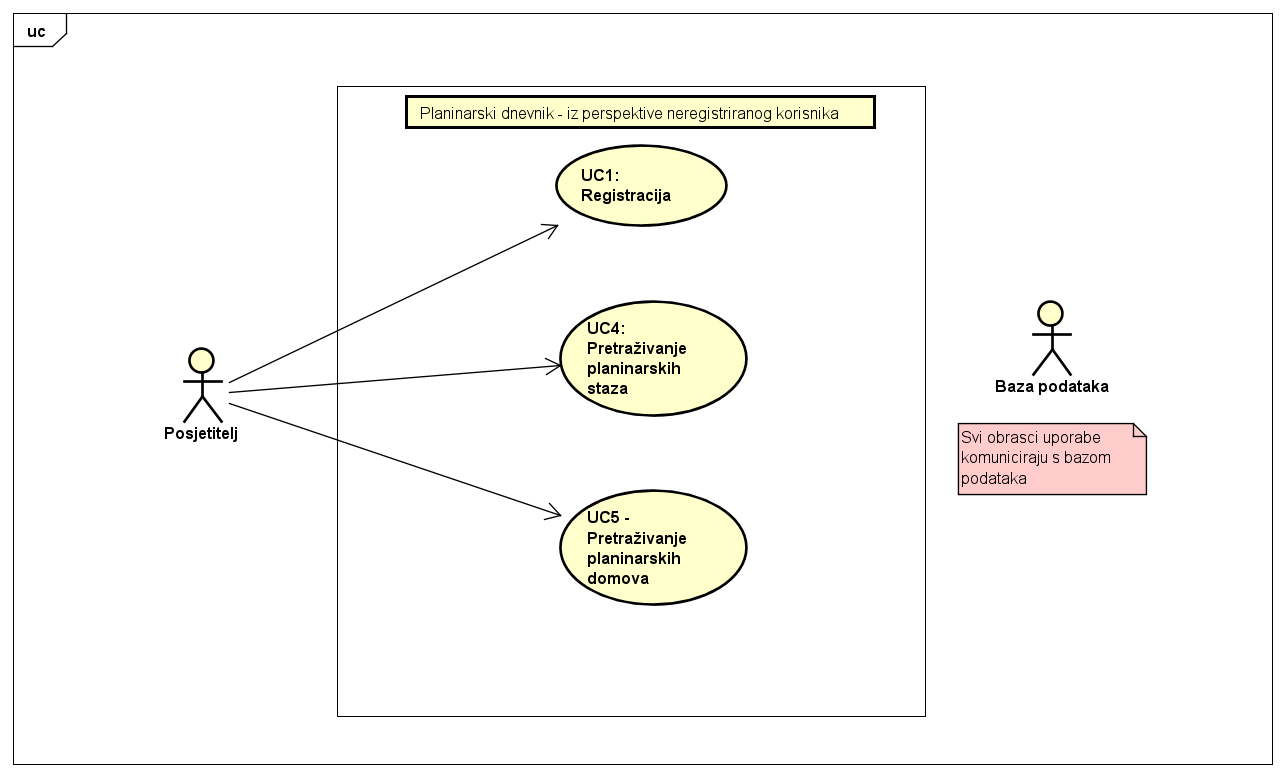
\includegraphics[scale=0.5]{dijagrami/posjetitelj-funkcionalnosti.png} %veličina slike u odnosu na originalnu datoteku i pozicija slike
					\centering
					\caption{Prikaz funkcionalnosti dostupnih neregistriranom ili neprijavljenom korisniku}
					\label{fig:UC dijagrami}
				\end{figure}
		
			\begin{figure}[H]
				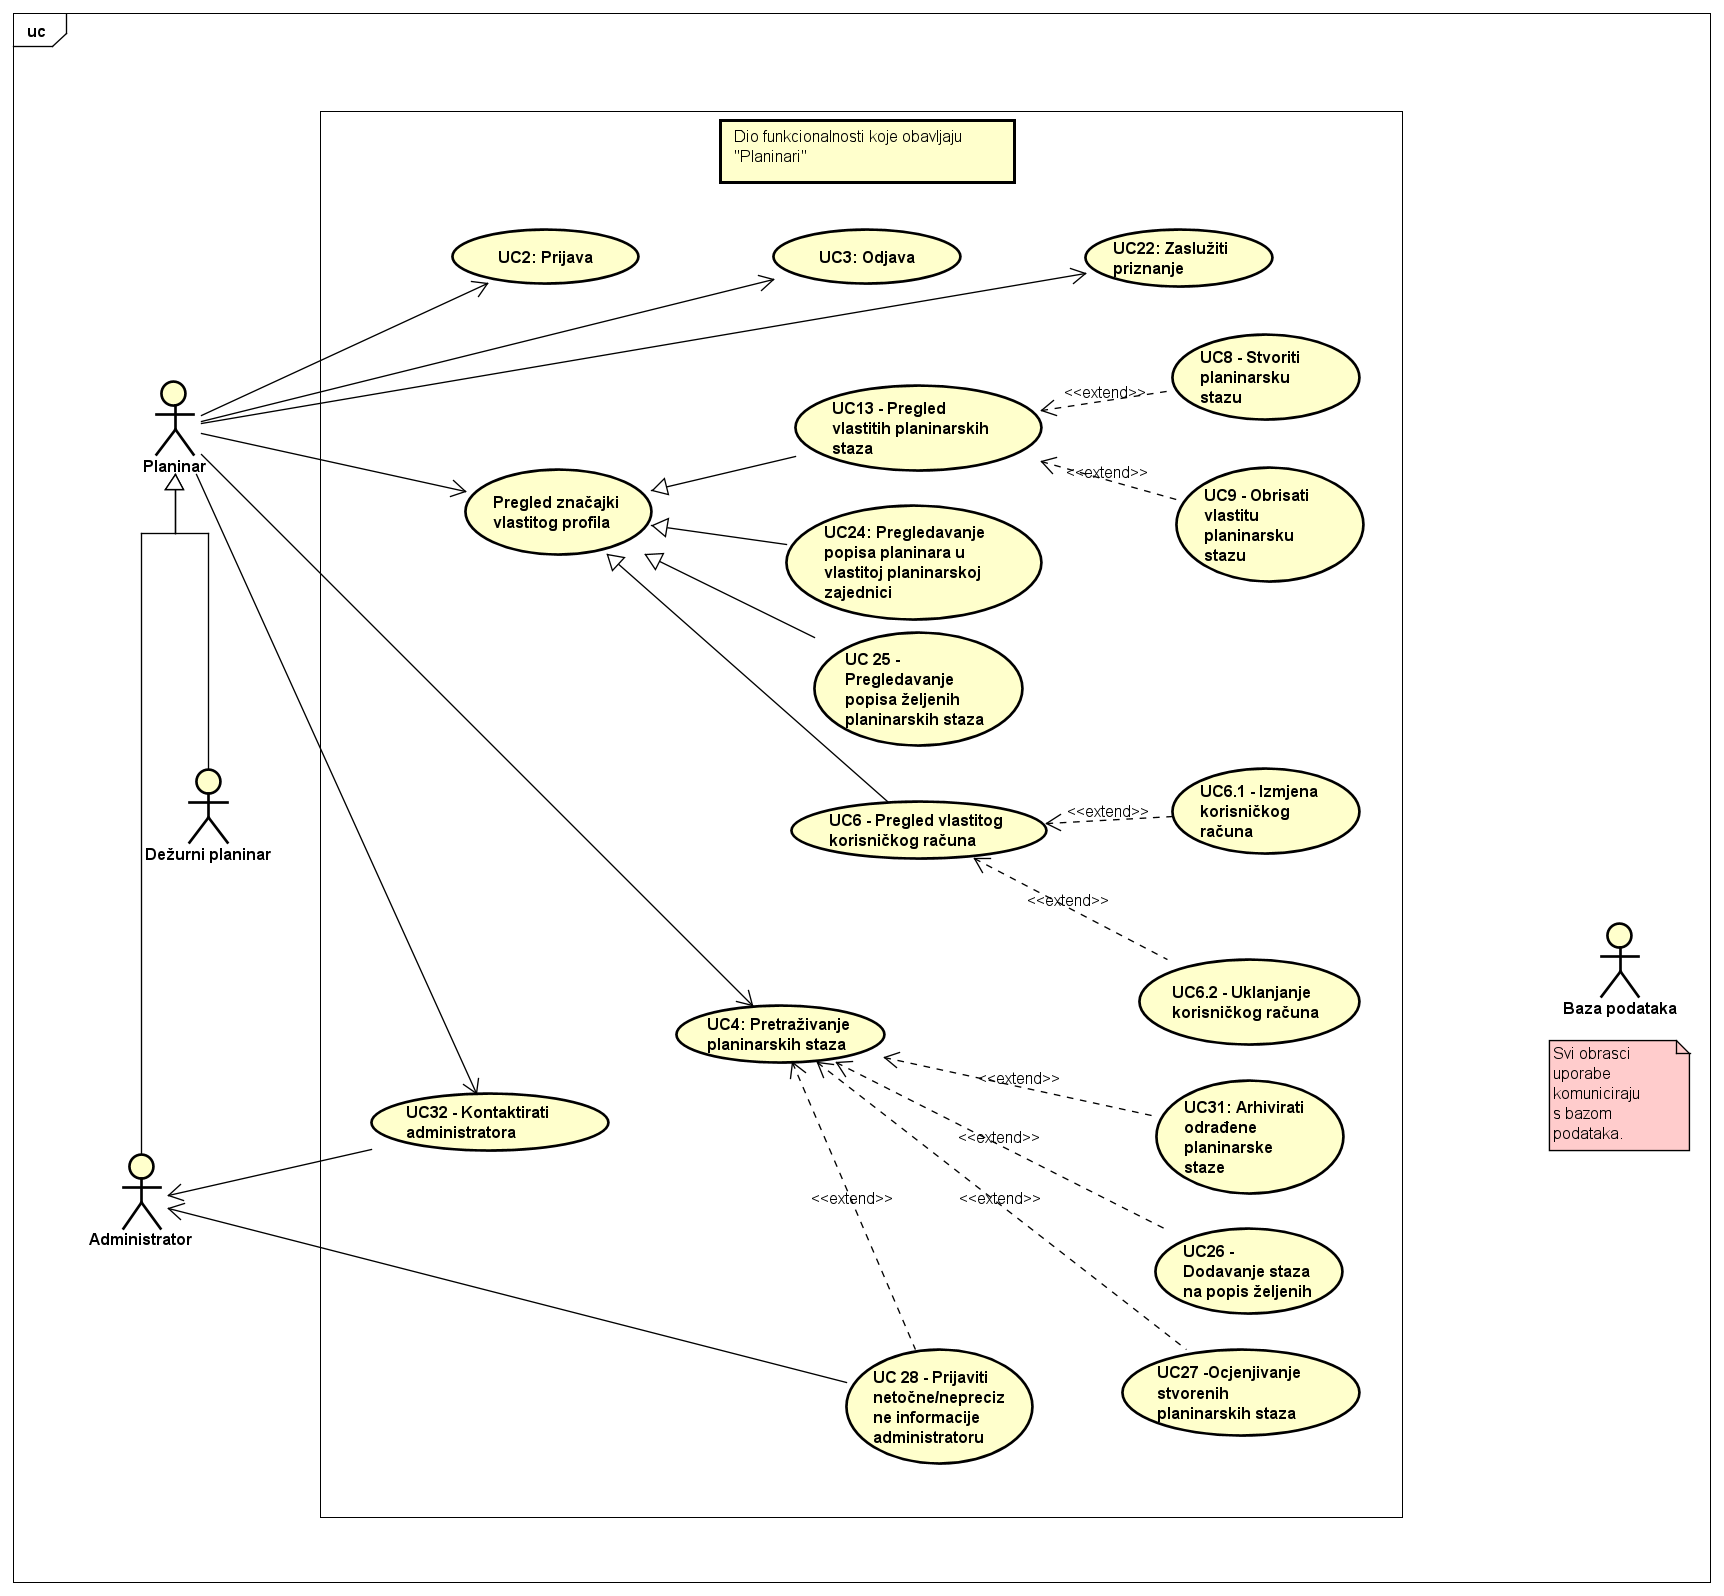
\includegraphics[scale=1, width = 165mm, height=220mm]{dijagrami/planinar1.png} %veličina slike u odnosu na originalnu datoteku i pozicija slike
				\centering
				\caption{Dio funkcionalnosti koje obavljaju planinari}
				\label{fig:UC dijagrami}
			\end{figure}
	
			\begin{figure}[H]
				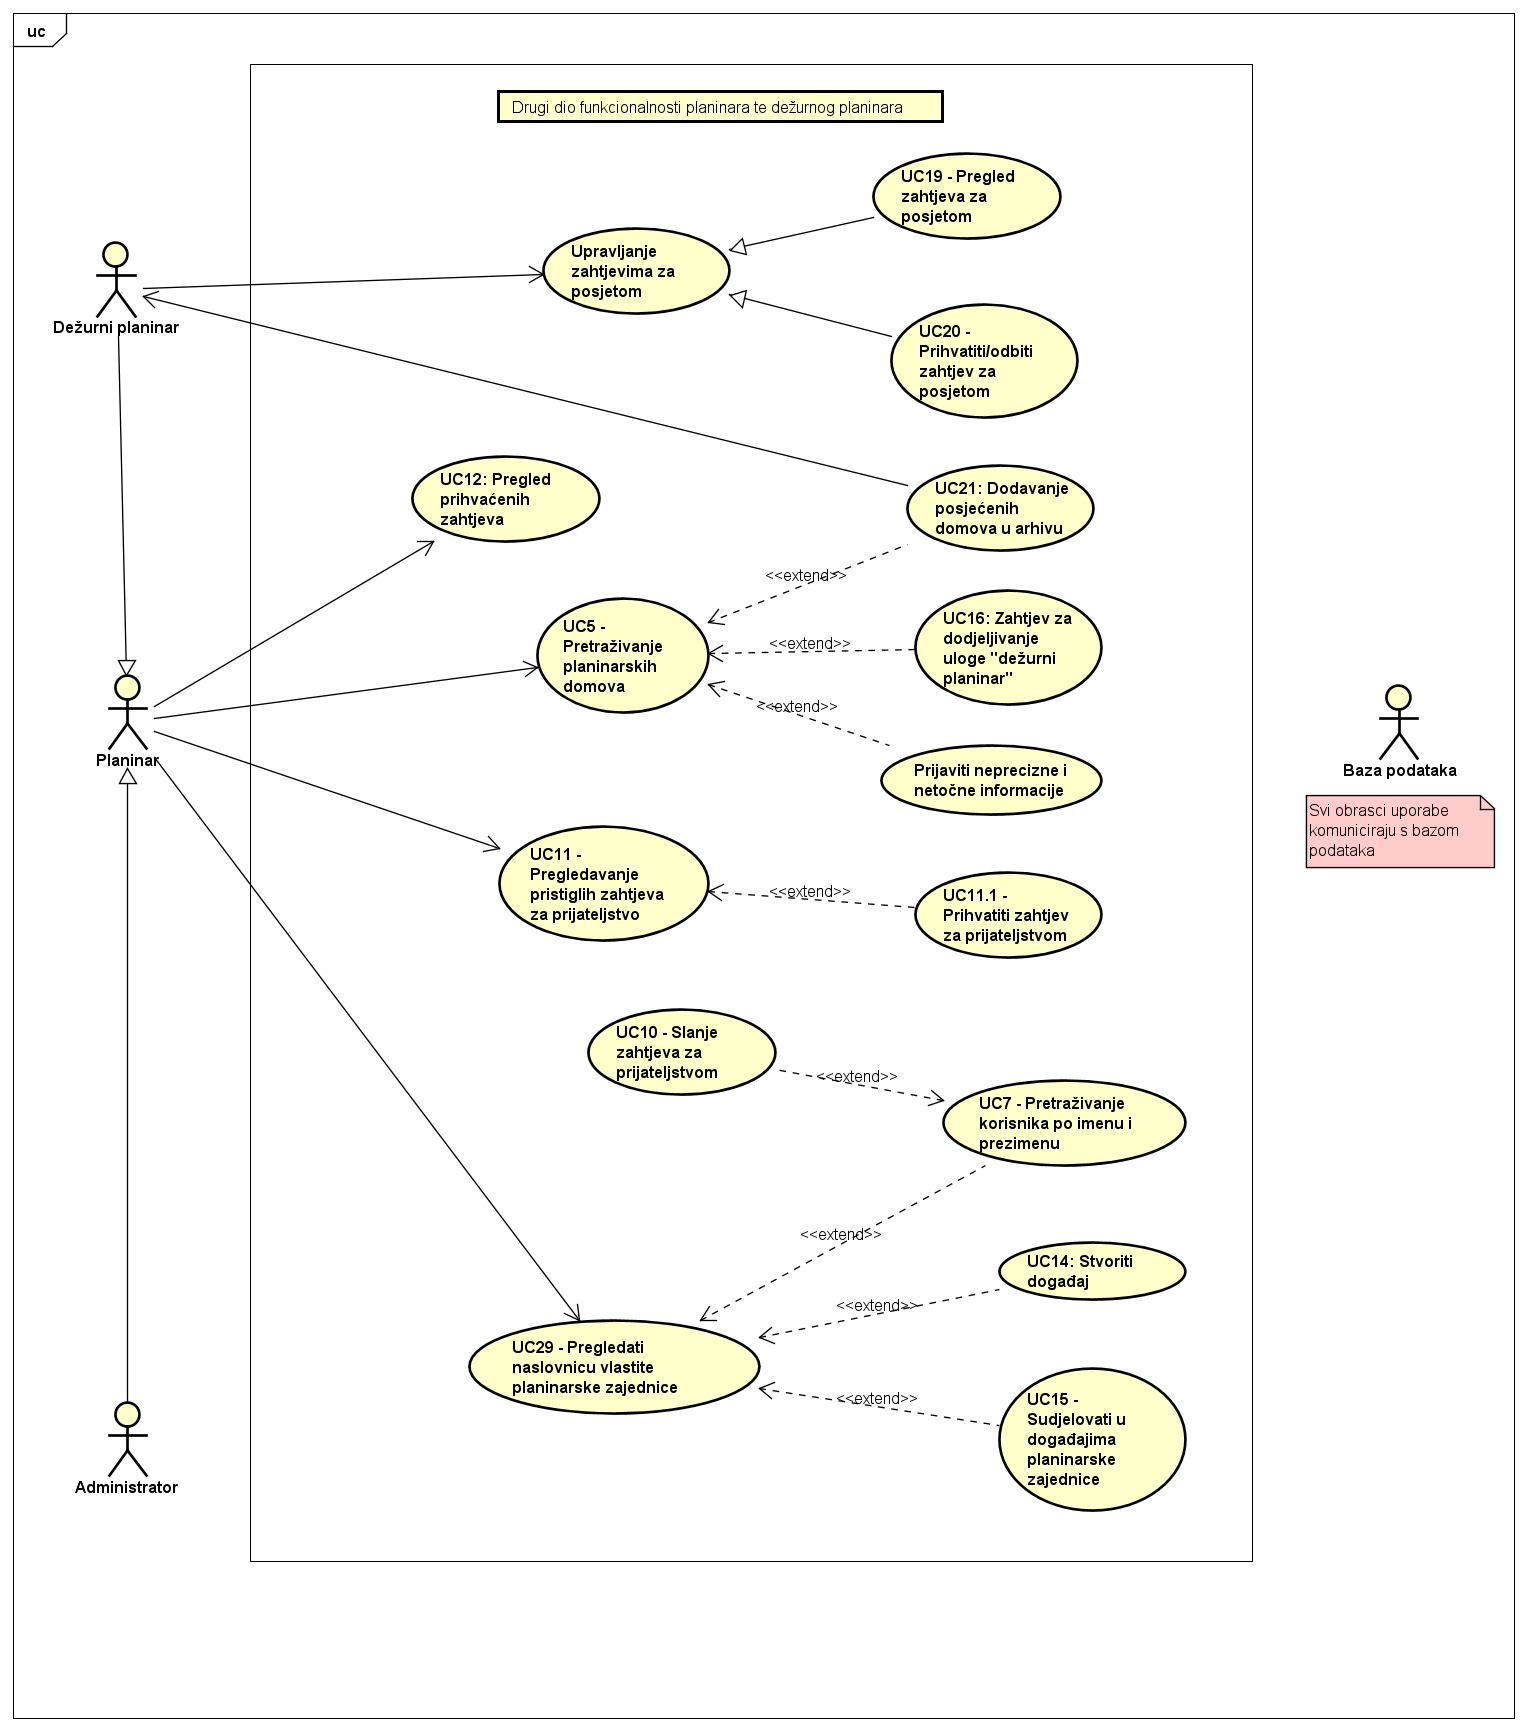
\includegraphics[scale=1, width = 165mm, height=220mm]{dijagrami/planinar2.png} %veličina slike u odnosu na originalnu datoteku i pozicija slike
				\centering
				\caption{Drugi dio funkcionalnosti planinara te zasebne aktivnosti dežurnog planinara}
				\label{fig:UC dijagrami}
			\end{figure}

		\begin{figure}[H]
			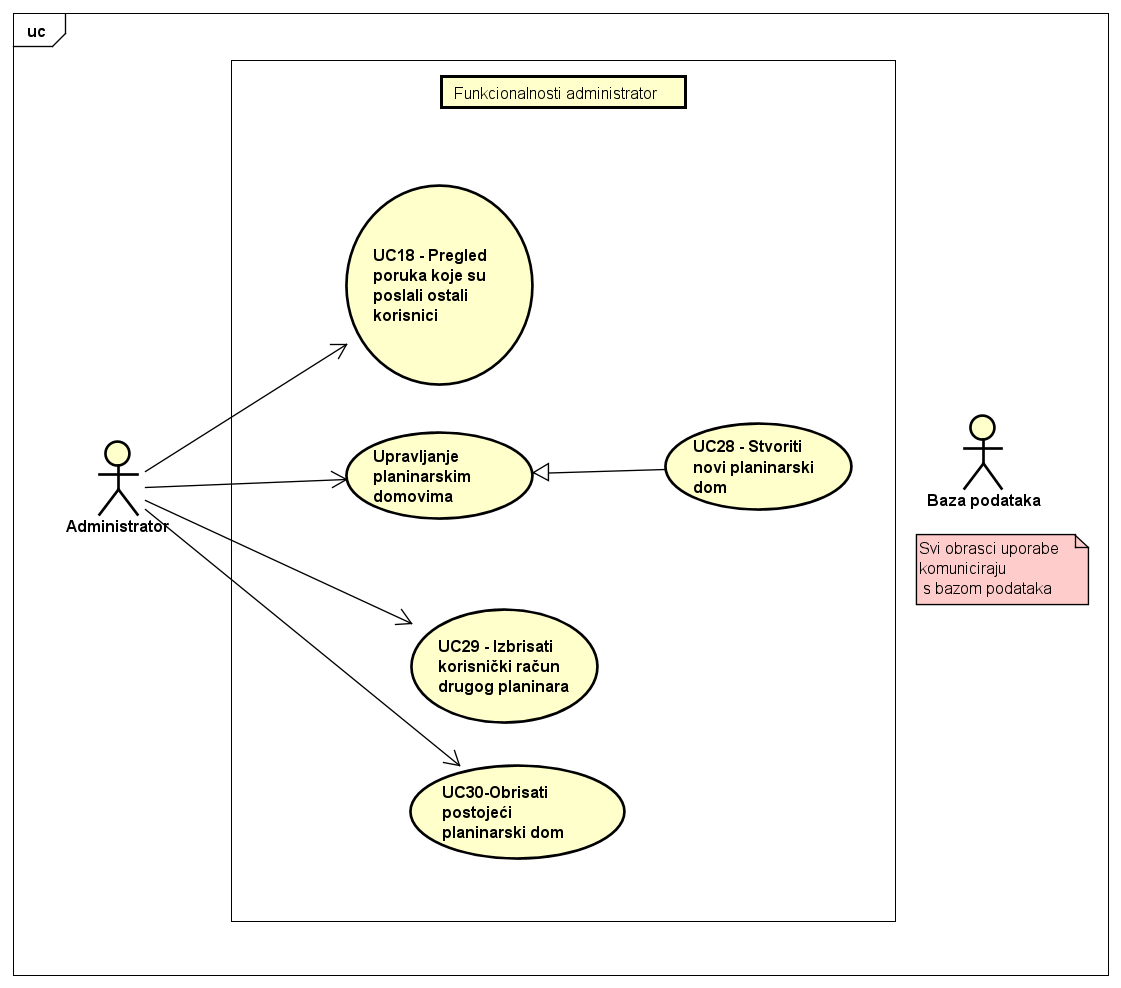
\includegraphics[scale=0.5]{dijagrami/administrator-funkcionalnosti.png} %veličina slike u odnosu na originalnu datoteku i pozicija slike
			\centering
			\caption{Prikaz funkcionalnosti koje obavlja administrator}
			\label{fig:UC dijagrami}
		\end{figure}
				
				
			\newpage	
				
			\subsection{Sekvencijski dijagrami}
			
			\subsubsection{Obrazac uporabe UC5 - Pretraživanje planinarskih domova}
			
			Korisnik odabire funkciju pregleda svih planinarskih domova. Web aplikacija, na traženi zahtjev, dohvaća planinarske domove iz baze podataka. Baza podataka zatim šalje odgovor Web aplikaciji. Odgovor baze podataka web aplikacija prikazuje korisniku. Nadalje, ako korisnik želi užu pretragu               planinarskih domova, odabire jedan od filtera koje aplikacija nudi. Web aplikacija dohvaća iz baze podataka planinarske domove koji zadovoljavaju filtere korisnika. Baza podataka šalje listu odgovarajućih domova aplikaciji. U slučaju da je lista prazna, web aplikacija korisniku šalje povratnu informaciju o nepostojećem domu. Ako su odgovarajući domovi pronađeni u bazi podataka web aplikacija prikazuje listu planinarskih domova korisniku. 
				
				\begin{figure}[H]
					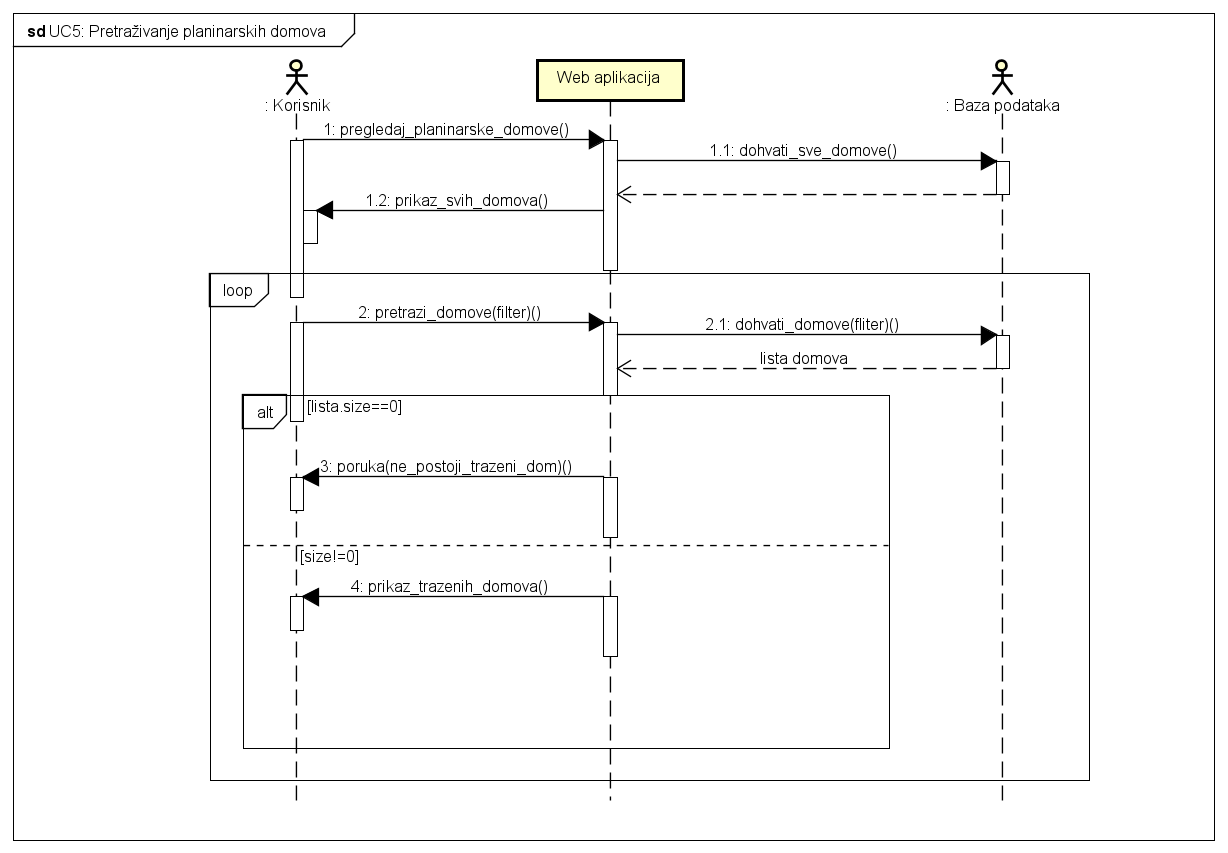
\includegraphics[scale=0.5]{dijagrami/seq-planinarski-domovi.png} %veličina slike u odnosu na originalnu datoteku i pozicija slike
					\centering
					\caption{Ponašajni prikaz pretraživanja planinarskih domova}
					\label{fig:UC dijagrami}
				\end{figure}
				
			

				\subsubsection{Obrazac uporabe UC9 - Obrisati vlastitu planinarsku stazu}

				Prijavljeni korisnik (planinar) na vlastitom profilu ima mogućnost pregleda popisa svih staza koje je stvorio. Odabirom opcije ''Moje staze'' planinar šalje zahtjev poslužitelju za prikaz tih staza. Poslužitelj dohvaća sve njegove staze iz baze podataka i prikazuje ih planinaru na njegovom profilu. Planinar zatim može odabrati stazu koju želi ukloniti tako što odabere opciju ''Ukloni stazu''. Poslužitelj u bazi podataka provjerava vidljivost odabrane staze, odnosno je li ona javna ili privatna.  Ako u bazi podataka za odabranu stazu vrijedi da je javna, onda će korisnik od poslužitelja primiti poruku da je stazu nemoguće ukloniti. Inače, ako je staza privatna, poslužitelj će korisniku postaviti pitanje: ''Jeste li sigurni da želite ukloniti stazu?'' na što planinar može odgovoriti potvrdno ili odustati od brisanja. U slučaju potvrdnog odgovora, kojeg planinar šalje poslužitelju, poslužitelj će narediti bazi podataka da ukloni odabranu stazu s popisa staza i vratit će se odgovor prema planinaru da je staza uspješno uklonjena. Ako planinar odustane od brisanja, sustav će ga vratiti na popis vlastitih staza. 

				\begin{figure}[H]
					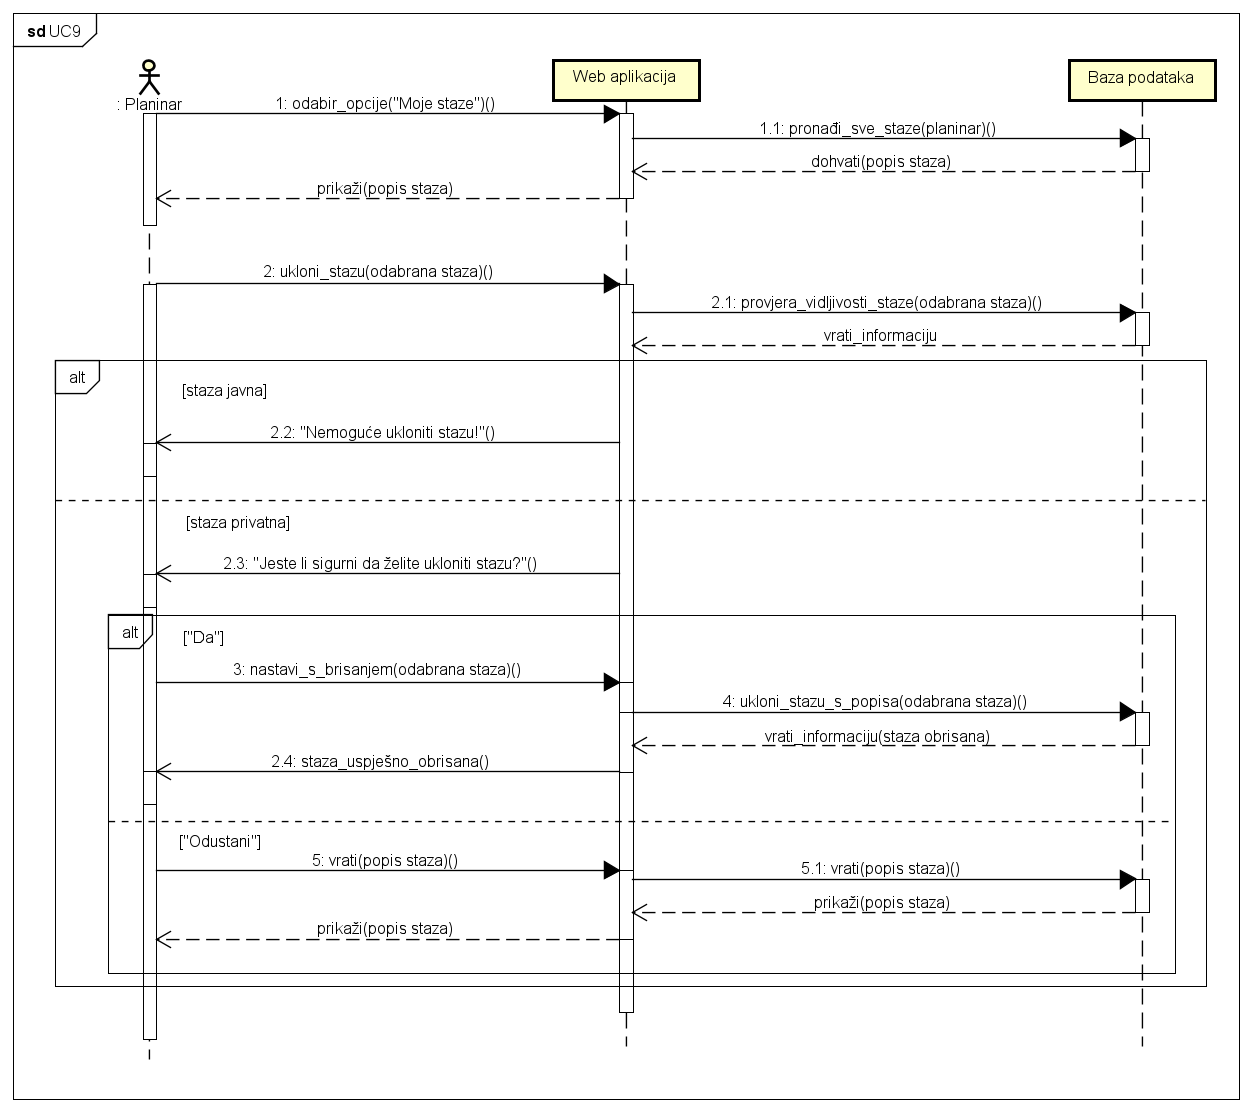
\includegraphics[scale=1.5, width=165mm, height=190mm]{dijagrami/seq-UC9.png} %veličina slike u odnosu na originalnu datoteku i pozicija slike
					\centering
					\caption{Sekvencijski dijagram za UC9}
					\label{fig:sekvencijski dijagrami}
				\end{figure}
				\newpage
				\subsubsection{Obrasci uporabe UC10-UC11-UC11.1 - Zahtjevi za prijateljstvom}

				Prijavljeni korisnik (planinar) može drugom korisniku poslati zahtjev za pridruživanjem vlastitoj planinarskoj zajednici, odnosno zahtjev za prijateljstvom. Uvjet je da pošiljatelj i primatelj (planinari) imaju korisnički račun, drugim riječima da su se uspješno registrirali u aplikaciju. Planinar ima mogućnost pretraživanja drugih planinara po imenu i prezimenu. Poslužitelj će tu pretragu proslijediti bazi podataka koja će pronaći sve korisnike koji zadovoljavaju pretragu. Baza podataka vraća odgovarajuće korisnike poslužitelju koji ih onda prikazuje planinaru. Zatim planinar pošiljatelj odabire planinara iz prikazanih mu korisnika i odluči mu poslati zahtjev za prijateljstvom. Bilo koji planinar prijavljen u aplikaciju može vidjeti sve trenutno aktivne zahtjeve za prijateljstvo. U našem slučaju planinar primatelj može ili dobiti obavijest da je primio zahtjev ili može zatražiti pregled pristiglih zahtjeva. Kada planinar prima novi zahtjev poslužitelj prolongira zahtjev do planinara primatelja i vraća se povratna informacija do planinara pošiljatelja da je zahtjev uspješno poslan. Za to vrijeme u bazu podataka će se dodati taj zahtjev među aktivne zahtjeve za prijateljstvom. Ako planinar sam zatraži pregled svih zahtjeva to će napraviti tako da kontaktira poslužitelja koji će naredbu proslijediti bazi podataka. Baza podataka će tada dohvatiti aktivne zahtjeve za prijateljstvo i poslati ih poslužitelju koji će ih konačno prikazati planinaru. Planinar primatelj kod obrađivanja primljenog zahtjeva za prijateljstvo ima dvije mogućnosti: potvrditi ili odbiti zahtjev. U slučaju povrđivanja zahtjeva planinar primatelj će poslati potvrdu poslužitelju  koji će javiti planinaru primatelju da je prihvaćen njegov zahtjev za prijateljstvo. Istovremeno baza podataka će ukloniti zahtjev s popisa aktivnih zahtjeva. Ukoliko planinar primatelj odluči odbiti zahtjev, onda se taj zahtjev također uklanja s popisa aktivnih zahtjeva u bazi podataka i planinar pošiljatelj može ponovno poslati zahtjev tom istom planinaru koji ga je već odbio.
				
				\begin{figure}[H]
					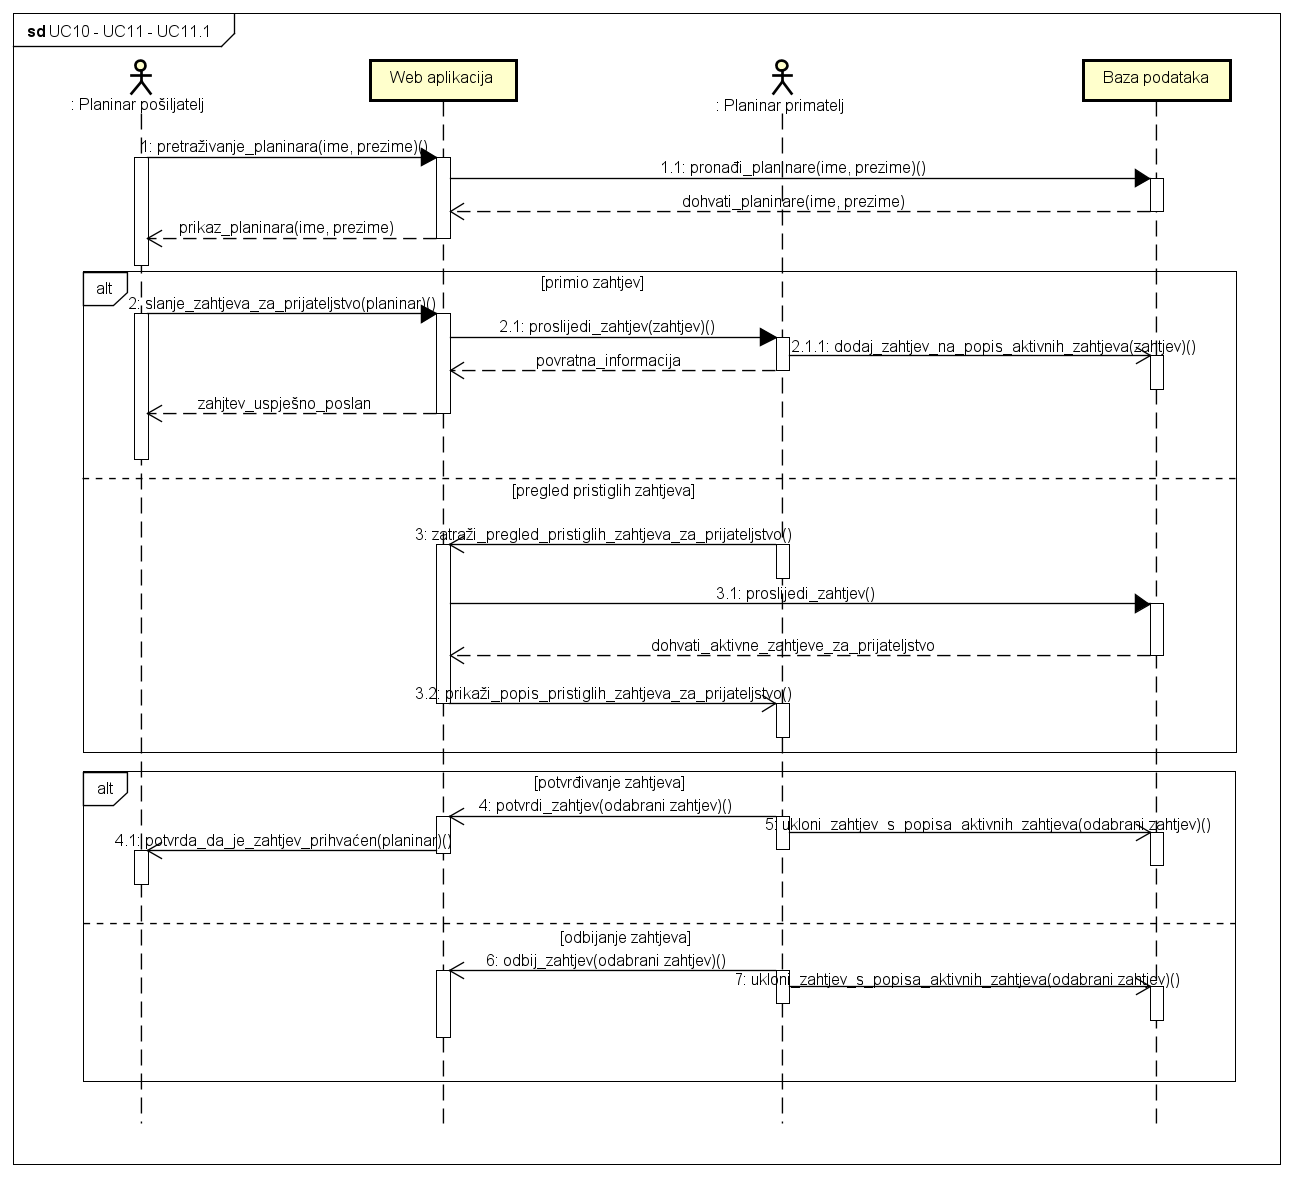
\includegraphics[scale=1.5, height=220mm, width=165mm]{dijagrami/seq-UC10 - UC11 - UC11.1.png} %veličina slike u odnosu na originalnu datoteku i pozicija slike
					\centering
					\caption{Sekvencijski dijagram za UC10 - UC11 - UC11.1}
					\label{fig:sekvencijski dijagrami}
				\end{figure}

				\eject
		\section{Ostali zahtjevi}
		
		 
			 	\begin{packed_item}
			 	
			 	\item  $ $Sustav treba omogućiti rad više korisnika u stvarnom vremenu $ $
			 	\item  $ $Sustav treba biti implementiran kao web aplikacija koja će biti prilagođena i prikazu na mobilnim uređajima (aplikacija mora imati responzivan dizajn) $ $
			 	\item  $ $Korisnicima korištenje aplikacije treba biti intuitivno jasno, bez potrebe za dodatnim korisničkim uputama$ $
			 	\item  $ $Korisničko sučelje i sustav trebaju koristiti hrvatski standardni jezik (uključujući dijakritičke znakove)$ $
			 	\item  $ $Eventualne pogreške korisnika i/ili administratora ne smiju utjecati na uspješno funkcioniranje aplikacije$ $
			 	\item  $ $Baza podataka treba biti brza, učinkovita i dobro povezana sa sustavom, otporna na bilo kakve greške korisnika i administratora $ $
			 	
			 	\item  $ $Aplikacija mora biti dostupna svim zainteresiranim korisnicima, odnosno svim već aktivnim planinarima, ali i onima koji to tek namjeravaju postati$ $
			 	\item  $ $Korisnik sustavu treba moći pristupiti iz javne mreže pomoću protokola HTTPS $ $
			 	\item  $ $Nadogradnja sustava ne smije narušavati postojeće funkcionalnosti sustava$ $
			 	
			 
			 \end{packed_item}
			 
			 \eject
			 
	